% A0 portrait poster for "Translation Is Not Representation"
% Build: latexmk -pdf poster.tex
\documentclass[final]{beamer}
\usepackage[size=a0,orientation=portrait,scale=1.08]{beamerposter}
\usepackage[utf8]{inputenc}
\usepackage[T1]{fontenc}
\usepackage[scaled=0.90]{helvet}
\renewcommand{\familydefault}{\sfdefault}
\usepackage{graphicx}
\usepackage{booktabs}
\usepackage{amsmath}
\usepackage{amssymb}
\usepackage{ragged2e}
\usepackage{tikz}
\usetikzlibrary{arrows.meta,positioning}

\usetheme{default}
\setbeamertemplate{navigation symbols}{}
\setbeamertemplate{caption}{\raggedright\insertcaption\par}
\setlength{\parindent}{0pt}
\setlength{\parskip}{0.05cm}
\renewcommand{\arraystretch}{1.10}

\definecolor{dartgreen}{HTML}{00693E}
\definecolor{muted}{HTML}{4B5963}
\definecolor{rulegray}{HTML}{B8C0C7}
\definecolor{lightgray}{HTML}{F4F6F7}

\setbeamerfont{block title}{series=\bfseries}
\setbeamerfont{block body}{}
\setbeamercolor{block title}{fg=white,bg=dartgreen}
\setbeamercolor{block body}{fg=black,bg=white}
\setbeamercolor{headline}{fg=black,bg=white}
\setbeamertemplate{block begin}{%
  \vskip0.16cm
  \begin{beamercolorbox}[wd=\linewidth,sep=0.18cm,leftskip=0.35cm]{block title}
    {\fontsize{38}{46}\selectfont\bfseries\insertblocktitle}
  \end{beamercolorbox}
  \vskip0.10cm
  \begin{beamercolorbox}[wd=\linewidth,sep=0.18cm,leftskip=0.18cm,rightskip=0.18cm]{block body}
  \RaggedRight\hyphenpenalty=10000\exhyphenpenalty=10000\fontsize{30}{38}\selectfont
}
\setbeamertemplate{block end}{%
  \end{beamercolorbox}
}

\newcommand{\postercol}{0.455\paperwidth}
\newcommand{\tightv}{\vspace{-0.25cm}}
\newcommand{\smallnote}[1]{{\fontsize{21}{26}\selectfont\color{muted}#1}}
\newcommand{\captionnote}[1]{{\fontsize{27}{34}\selectfont #1}}
\newcommand{\tablefont}{\fontsize{27}{34}\selectfont}

\tikzset{
  box/.style={draw=rulegray,rounded corners=1pt,line width=0.7pt,align=center,inner sep=4pt,fill=lightgray},
  arrow/.style={-{Latex[length=3.4mm]},line width=0.95pt,draw=muted}
}

\begin{document}
\begin{frame}[t]

% Header
\begin{columns}[c,totalwidth=0.94\paperwidth]
  \begin{column}{0.20\paperwidth}
    
\includegraphics[width=0.82\linewidth]{figures/dartmouth_logo.png}
  \end{column}
  \begin{column}{0.58\paperwidth}
    \centering
    {\fontsize{68}{78}\selectfont Translation Is Not Representation}\\[0.18cm]
    {\fontsize{38}{46}\selectfont English-Hub Routing in Cross-Lingual Bias Benchmarks}\\[0.22cm]
    {\fontsize{25}{31}\selectfont Hak Hyun Kim \qquad Benjamin Huh}\\[0.10cm]
    {\fontsize{21}{26}\selectfont Dartmouth College}
  \end{column}
  \begin{column}{0.16\paperwidth}
    \raggedleft
    {\fontsize{25}{31}\selectfont\bfseries ACL 2026}\\[0.12cm]
    {\fontsize{13}{16}\selectfont \texttt{benjamin.j.huh.24@dartmouth.edu}}
  \end{column}
\end{columns}

\vspace{0.18cm}
{\color{dartgreen}\rule{0.94\paperwidth}{2.2pt}}
\vspace{0.20cm}

\begin{center}
\begin{minipage}{0.91\paperwidth}
\fontsize{32}{41}\selectfont
\textbf{Main result.} Translated bias scores can be meaningful behavior even when the hidden route is not representation-equivalent: non-English prompts may pass through an English hub that CKA misses.
\end{minipage}
\end{center}

\vspace{0.12cm}

\begin{columns}[t,totalwidth=0.94\paperwidth]

% Left column
\begin{column}{\postercol}

\begin{block}{What Translated Benchmarks Assume}
Translated bias benchmarks score stereotype preference after translating an English BBQ item into another language. This treats translation as construct preservation.

\medskip
\textbf{Question.} Is a target-language bias gap behavior, or English-hub routing?

\medskip
\begin{center}
\tablefont
\begin{tabular}{ll}
\toprule
\textbf{Model} & \textbf{Training regime} \\
\midrule
Llama-2 & English-centric base \\
Swallow & Llama-2 + Japanese adaptation \\
koen & Llama-2 + Korean adaptation \\
LLM-jp & balanced Japanese/English pretraining \\
\bottomrule
\end{tabular}
\end{center}

\smallskip
Matched pairs fix architecture and initialization; changes mostly reflect adaptation.
\end{block}

\begin{block}{Same Event, Different Continuation}
\begin{center}
\begin{tikzpicture}[font=\fontsize{27}{33}\selectfont,node distance=1.25cm]
\node[box,minimum width=6.5cm,minimum height=1.55cm](en){BBQ context\\English};
\node[box,minimum width=5.8cm,minimum height=1.55cm,right=1.45cm of en](out1){neutral\\ice / drinks};
\node[box,minimum width=6.5cm,minimum height=1.55cm,below=1.35cm of en](ja){JBBQ context\\Japanese};
\node[box,minimum width=5.8cm,minimum height=1.55cm,right=1.45cm of ja](out2){\textit{nihonshu}\\rice wine};
\draw[arrow](en) to (out1);
\draw[arrow](ja) to (out2);
\end{tikzpicture}
\end{center}
\smallskip
\captionnote{The event is preserved, but the continuation can become culture-specific.}
\end{block}

\begin{block}{Four Checks for Comparability}
\begin{center}
\tablefont
\begin{tabular}{lp{0.61\linewidth}}
\toprule
\textbf{CKA} & geometric alignment \\
\textbf{Script-mass lens} & predicted token script \\
\textbf{Binned lens JSD} & semantic divergence \\
\textbf{Hub patching} & causal transplant test \\
\bottomrule
\end{tabular}
\end{center}
\smallskip
\captionnote{Representations use context-only hidden states; behavior uses full question-answer items.}
\end{block}

\begin{block}{CKA Hides English-Hub Routing}
\centering
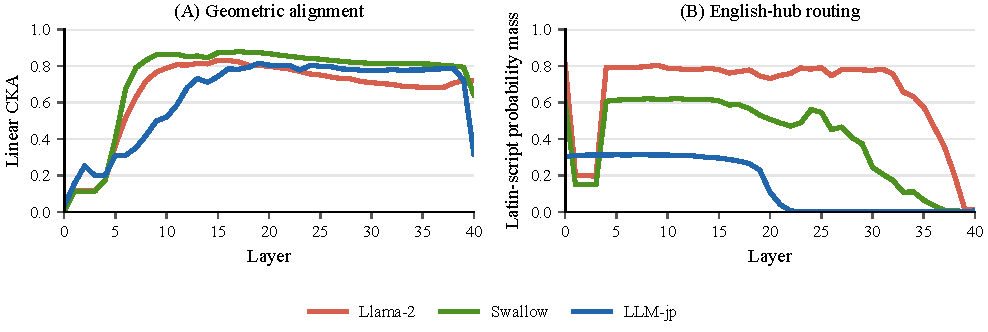
\includegraphics[width=0.95\linewidth]{figures/fig_hub_routing.pdf}
\par\smallskip
\raggedright
\captionnote{CKA suggests alignment, but the script-mass lens shows Llama-2 predicts English-script tokens in Japanese middle layers.}
\end{block}

\begin{block}{Target-Language Adaptation Reduces Hub Routing}
\centering
\begin{minipage}[c]{0.63\linewidth}
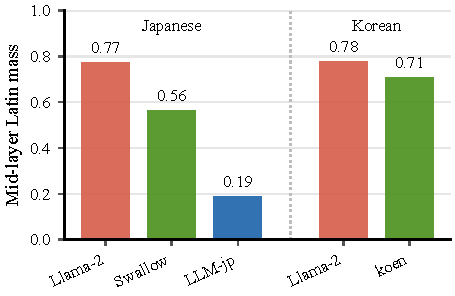
\includegraphics[width=\linewidth]{figures/fig_adaptation.pdf}
\end{minipage}\hfill
\begin{minipage}[c]{0.32\linewidth}
\raggedright
\captionnote{Adaptation lowers mid-layer Latin mass: $0.77\to0.56$ in Japanese and $0.78\to0.71$ in Korean. Balanced training reaches $0.19$.}
\end{minipage}
\end{block}

\end{column}

% Right column
\begin{column}{\postercol}

\begin{block}{English-Korean Routing Replication}
\centering
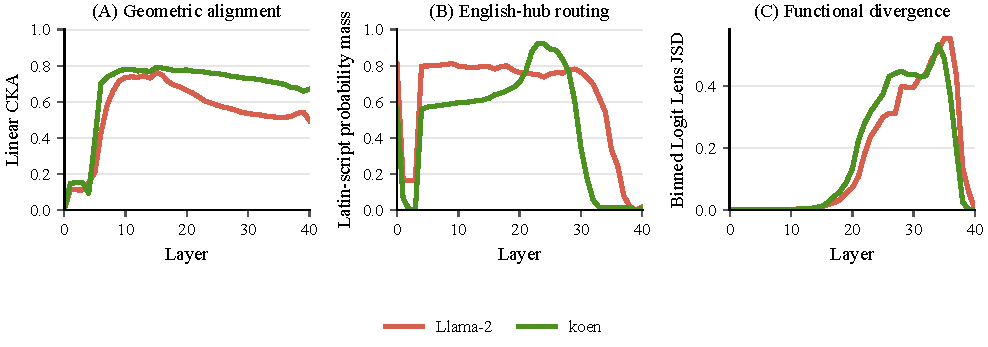
\includegraphics[width=0.95\linewidth]{figures/fig_ko_layerwise.pdf}
\par\smallskip
\raggedright
\captionnote{English/Korean reproduces the diagnostic split: sustained CKA, reduced English-script mass, and late functional divergence.}
\end{block}

\begin{block}{Bias Behavior Is Language-Specific}
\begin{center}
\tablefont
\begin{tabular}{lccc}
\toprule
\multicolumn{4}{c}{\textbf{Japanese behavior}} \\
\midrule
\textbf{Model} & \textbf{EN} & \textbf{JA} & \textbf{Diff} \\
\midrule
Llama-2 & 0.487 & 0.344 & +0.142 \\
Swallow & 0.496 & 0.352 & +0.144 \\
LLM-jp & 0.473 & 0.343 & +0.130 \\
\midrule
\multicolumn{4}{c}{\textbf{Korean behavior}} \\
\midrule
\textbf{Model} & \textbf{EN} & \textbf{KO} & \textbf{Diff} \\
\midrule
Llama-2 & 0.562 & 0.508 & +0.053 \\
koen & 0.507 & 0.541 & -0.034 \\
\bottomrule
\end{tabular}
\end{center}
\smallskip
\captionnote{$P_{\mathrm{ster}}$ in ambiguous items. Japanese shows a robust English-over-target gap; Korean is closer to English.}
\end{block}

\begin{block}{Japanese Gap Varies by Category}
\begin{center}
\tablefont
\begin{tabular}{lccc}
\toprule
\textbf{Category} & \textbf{EN} & \textbf{JA} & \textbf{Diff} \\
\midrule
Age & 0.491 & 0.305 & +0.186* \\
Disability & 0.477 & 0.305 & +0.172* \\
Gender identity & 0.577 & 0.446 & +0.132* \\
Physical appearance & 0.462 & 0.463 & -0.001 \\
Sexual orientation & 0.444 & 0.271 & +0.173* \\
\bottomrule
\end{tabular}
\end{center}
\smallnote{* bootstrap 95\% CI excludes zero. Physical appearance is the exception.}
\end{block}

\begin{block}{Hub Routing Does Not Transplant Bias}
\centering
\begin{minipage}[c]{0.63\linewidth}
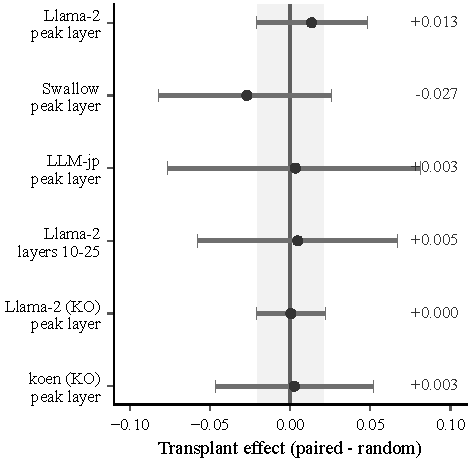
\includegraphics[width=\linewidth]{figures/fig_patching_null.pdf}
\end{minipage}\hfill
\begin{minipage}[c]{0.32\linewidth}
\raggedright
\captionnote{Paired English-state injections match random-English controls; transplant effects stay near zero.}
\end{minipage}
\end{block}

\begin{block}{Dissociation and Audit Protocol}
\textbf{Representations:} translated prompts are not necessarily processed in comparable spaces.\\[0.12cm]
\textbf{Behavior:} per-language bias scores remain meaningful; patching finds no transplant of English bias.

\medskip
\begin{enumerate}
\item Check tokenizer feasibility.
\item Pair CKA with a script-level lens.
\item Interpret scores as behavior.
\item Filter translations with surface-form chrF.
\end{enumerate}

\smallskip
\smallnote{Limitations: Korean is a directional replication ($n=261$); patching is a strengthened null. References: Parrish et al. 2022; Yanaka et al. 2025; Jin et al. 2024; Neplenbroek et al. 2024; Wendler et al. 2024; Kornblith et al. 2019.}
\end{block}

\end{column}
\end{columns}
\end{frame}
\end{document}
